\subsubsubsection{range\_check\_u32}

\hspace*{\fill}

\indent U32RangeCheckGate is a gate that can decompose a number into base B little-endian limbs.

The gate structure is like \figref{fig:range-check-u32}.

\begin{figure}[!ht]
    \centering
    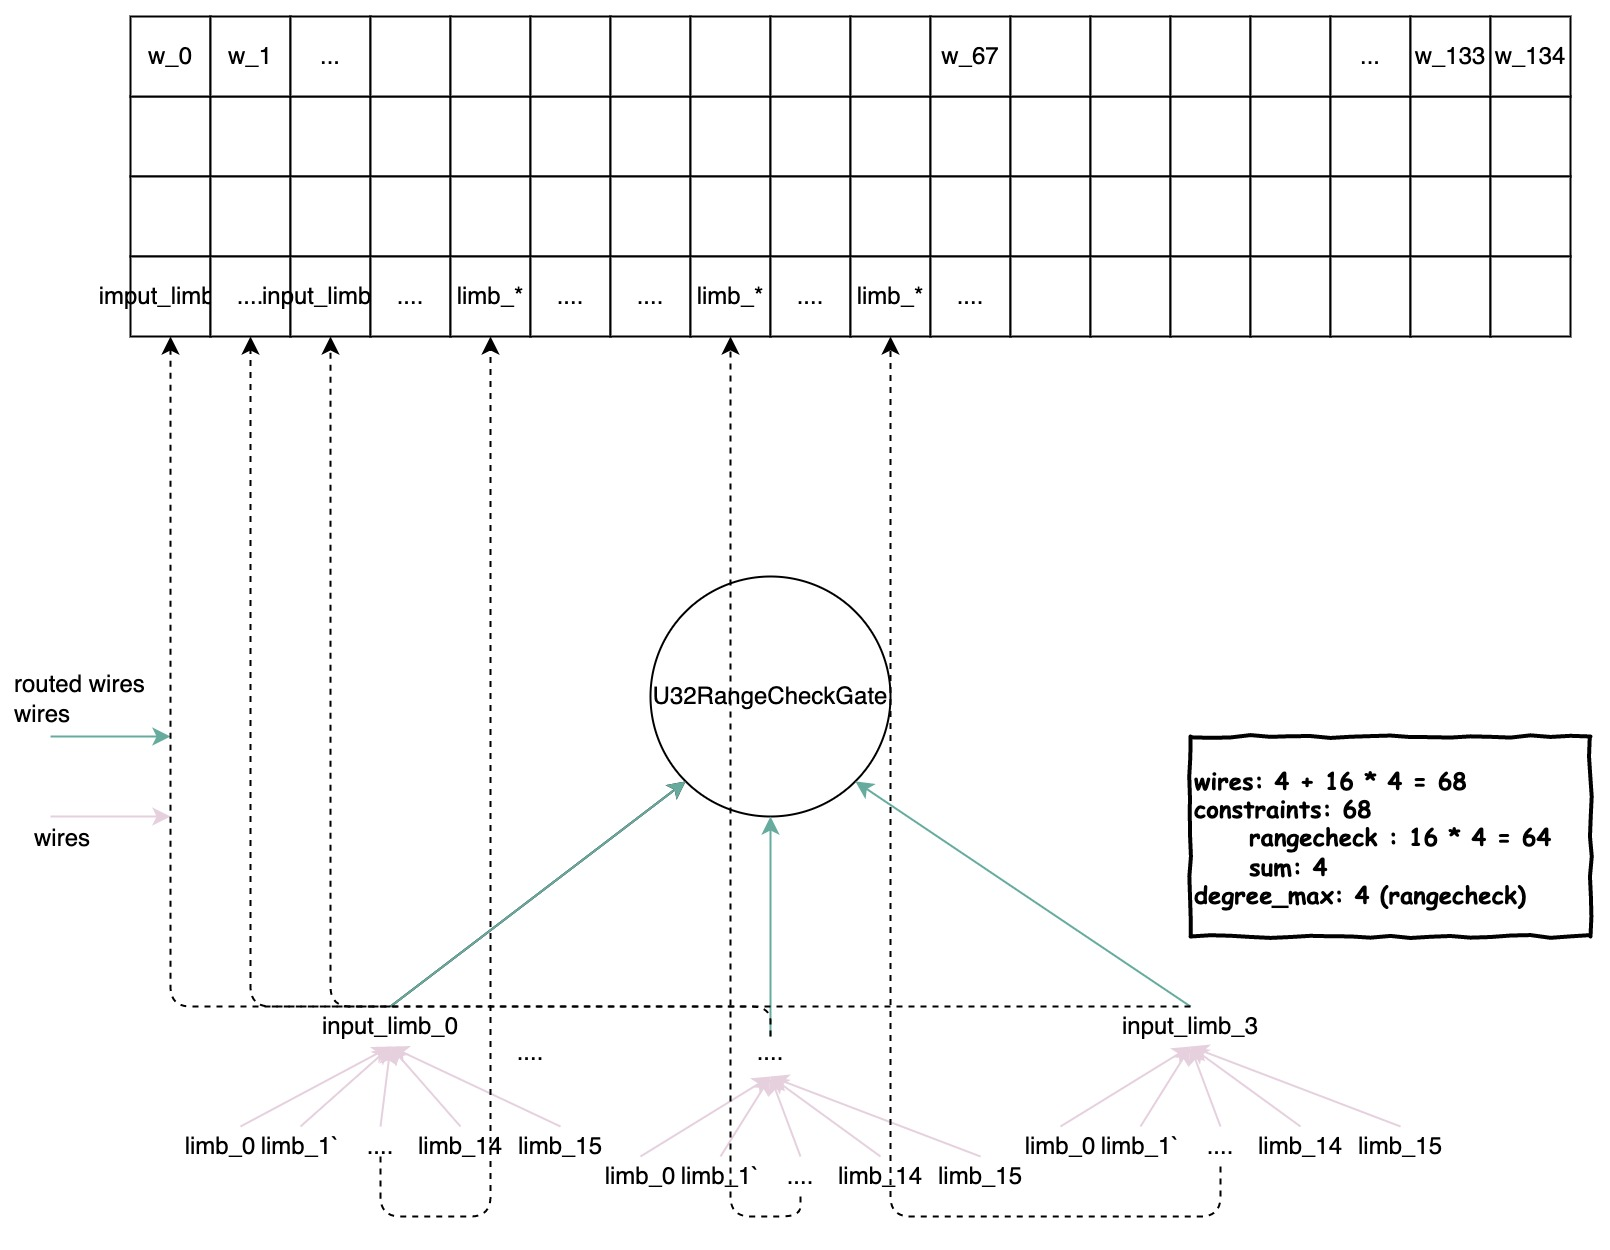
\includegraphics[width=0.6\textwidth]{gates/range_check_u32.jpeg}
    \caption{U32RangeCheckGate}
    \label{fig:range-check-u32}
\end{figure}

Constraints for each input\_limb:
\begin{itemize}
    \item Each input\_limb consists of its aux\_limbs. -- 1 constraint with degree 1.
    \begin{lstlisting}[language=rust]
let computed_sum = reduce_with_powers(&aux_limbs, base);
constraints.push(computed_sum - input_limb);
    \end{lstlisting}
    \item aux\_limbs range check. -- 16 (aux\_limbs) constraints with degree BASE ($(x-0)(x-1)\cdots(x-\text{BASE}+1)$).
\end{itemize}

In summary, there are 17 constraints per input limb, a total of $\text{num\_input\_limbs} \times 17$ constraints. 
The degree of the gate equals BASE for range check.
